\section{Data Analysis}

\subsection{Performance Metrics}
To interpret the results of the 3 models tested, it is important to first describe the various metrics used when evaluating a decision making system: precision, recall, F1 score, and accuracy. While accuracy is the easiest to understand, the ratio of the successes to all attempts, it does not provide as much insight into reliability. If a particular user encounters more spam than another, perhaps due to their email address being involved in a breach, then the same system may show a wildly different accuracy than that of a user receives very little spam. Many categorization systems will either handle false positives or false negatives better than the other, which is not reflected in the accuracy.

Instead, precision and recall are used to describe these facets of our detection system. Precision refers to, out of times where the system predicted a URL to be spam, the URL was indeed spam. Poor precision occurs when results identified as spam aren't usually spam, such as when benign URLs are misidientified more often the spam URLs are identified. If testing data contains significantly more safe URLs then spam URLs, precision is bound to be low, whereas precision is usually higher in datasets containing more spam than safe URLs. Recall instead refers to, out of the times where a piece of spam is evaluated, how frequently it is identified as such. Because recall only refers to data that is spam, the amount of spam relative to safe URLs in the dataset is not relevant, and recall is independent from that aspect of the sample.  The F1 score is a single metric that reflects both the precision and recall, which allows for both to be gleaned from a single statistic.

In addition to these metrics, which are commonly used to evaluate the performace of AI categorization models, it is also important to discuss performance metrics commonly associated with binary systems like this, such as false positive and false negative rate. Unlike precision and recall, both of these metrics are independent from the distrobution of the testing sample, allowing them to be more universally applicable. The false negative rate refers to, out of the URLs that are truly spam, how many were misidentified as safe; whereas the false positive rate refers to, out of the URLs that are truly safe, how many where misidentifies as spam.

There are two main reasons to split out false positive and false negative rates: to allow for predicting and simulating accuracy in systems given how much spam they are expected to see and to prioritize one rate over the other. For instance, if falsely identifying spam as safe just provides the receiver mild annoyance but falsely identifying a safe message as spam causing a critical message to be lost, than a system with a lower false positive rate would be desirable. However, if the system is just flagging messages as spam instead of hiding them, lower false negative rates might be more desireable.

\subsection{Results}

Of the three methods, using traditional AI performance metrics seen in figure \ref{fig:perf_metrics}, the random forest algorithm consistently outperformed the neural network, which in turn outperformed the K-Nearest Neightbor classifier. Across all methods, precision was at or above the recall, suggesting the models perform better with data that is safe rather than spam. Regardless, all of the metrics are close, and none of the methods have substantially poor performance in an area.

The false positive and false negative rates from figure \ref{fig:rate_metrics} show more descriptive data for these algorithms, though. For all three algorithms, the false positive rate is lower, again showing that the models do better on safe data. The random forest is much less susceptible to this trend, but still has a false negative rate over 1\% worse than its false positive rate. Whether or not this behavior is desireable depends on the particular implementation being used.

One naive way to improve the output of the algorithms would be to take input from all three. However, this would both incur a performance penalty and not result in significant improvement. If the three models were independent, such a technique could help, but they are not independent. URLs that are tougher for one model are likely also harder for another, as these harder URLs likely have some features of both safe and spam URLs. Rather, investigating these edge cases and improving one of the models has more potential than simplyed putting them together.

  \begin{figure}[!ht]
	\centering
	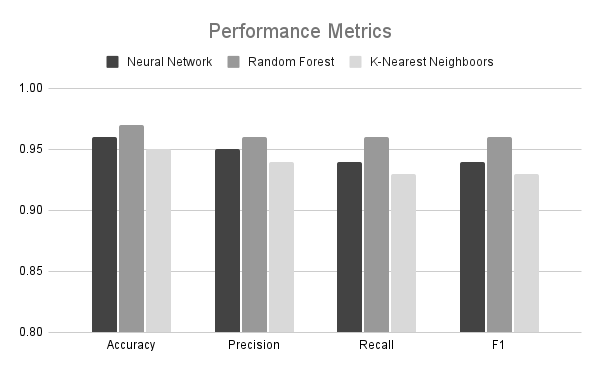
\includegraphics[width=3in]{Performance Metrics.png}
	
	\caption{\label{fig:perf_metrics} Performance results of the three models}
	
\end{figure}  
\begin{figure}[!ht]
\centering
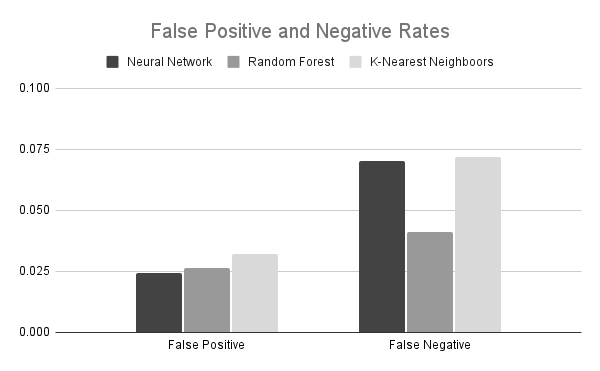
\includegraphics[width=3in]{False Positive and Negative Rates.png}

\caption{\label{fig:rate_metrics} Performance results of the three models}

\end{figure}

\subsection{Usage}

Using the URL's found in received emails is the primary use case for these models. More specifically, emails identified as spam may either be flagged to alert to user to the suspicious nature of the email or be outright discarded or hidden from the user. These two use cases have opposite needs with regard to false positives and false negatives. A legitimate email that is falsely identified as spam and thrown out could potentially cause serious issues for the sender or attempted recipient, leading to a need to lower false positives to near zero. Alternatively, if all the system does is add a banner at the top of the message warning the user, false positives are not harmful, and the potential damage from falling for a phishing attempt causes the balance to fall in the other direction.

As all of the discussed models have low error rates and very low false positive rates, more aggressive methods of hiding spam may be employed. Larger email providers can combine these systems with traditional methods, such as whitelists and blacklists for known good and bad domains, to help alleviate the remaining bad cases. These traditional methods generally perform worse on newer domains, leading to the concept of domain aging. Defering to AI to determine the trustworthyness of relatively young domains may help prevent false positives from recent registrations.


  